\documentclass{beamer}
%\usetheme{Boadilla}

\title{Bayesian Optimization}
\author{Steven}
\usepackage[utf8]{inputenc}
\usepackage{algpseudocode}
\usepackage{algorithm}
\usepackage[T1]{fontenc}
\usepackage{textcomp}
\usepackage[english]{babel}
\usepackage{verbatim}
\usepackage{cite}
%\setlist[enumerate]{ label=\arabic*.}


% Hide page number when page is empty
\usepackage{multicol}
\usepackage{xcolor}
% Other font I sometimes use.
% \usepackage{cmbright}

% Math stuff
\usepackage{amsmath, amsfonts, mathtools, amsthm, amssymb}
% Fancy script capitals
\usepackage{mathrsfs}
% Bold math
\usepackage{bm}


% Operators
\DeclareMathOperator{\Bd}{Bd}
\DeclareMathOperator{\Int}{Int}
\DeclareMathOperator{\cif}{if\;}

\DeclareMathOperator{\Var}{Var}
\DeclareMathOperator{\SD}{SD}
\DeclareMathOperator{\Cov}{Cov}
\DeclareMathOperator{\Cor}{Cor}
\DeclareMathOperator{\Pois}{Pois}
\DeclareMathOperator{\Dir}{Dir}
\DeclareMathOperator{\Unif}{Unif}
\DeclareMathOperator{\Gam}{Gamma}
\DeclareMathOperator{\Binom}{Binom}
\DeclareMathOperator{\Expo}{Expo}
\DeclareMathOperator{\dBeta}{dBeta}
\DeclareMathOperator{\tBeta}{tBeta}
\DeclareMathOperator{\Ber}{Ber}
\DeclareMathOperator{\IG}{IG}
\DeclareMathOperator{\Pb}{Pr}
\DeclareMathOperator*{\argmax}{arg\,max}
\DeclareMathOperator*{\argmin}{arg\,min}
\newcommand\deq{\stackrel{\mathclap{\tiny\mbox{d}}}{=}}
\def\bsy{\boldsymbol}



\begin{document}
\begin{frame}
    \titlepage
\end{frame}

\begin{frame}
    \frametitle{Motivation}
    \begin{centering}
        ``Why not the best?'' --Jimmy Carter
    \end{centering}
\end{frame}

\begin{frame}
    \frametitle{Optimization: Review}
    How to maximize differentiable $f:[a, b] \to \mathbb{R}$?
    \begin{enumerate}
        \item solve $f'(c) = 0$
            \pause
        \item check $f''(c) \leq 0$.
            \pause
        \item evaluate $f$ at $a$, $b$, and local maxes.
    \end{enumerate}
\end{frame}

\begin{frame}
    \frametitle{Model Problem: Baking}
    \begin{itemize}
        \item Unknown underlying behavior
            \pause
        \item Smooth underlying behavior
            \pause
        \item Expensive trials
            \pause
    \end{itemize}
    Solution: Iteratively sample $F$.
\end{frame}

\begin{frame}
    \frametitle{Algorithm: Overview}
    Given function unknown $F: \mathcal{X} \subseteq \mathbb{R}^{K} \to \mathbb{R}$, do the following loop
    \begin{enumerate}
        \item Given our observations about $F$, pic $\mathbf{x} \in \mathcal{X}$ with the most ``utility''.
            \pause
        \item Sample $F(\mathbf{x})$
            \pause
        \item Update our observations
            \pause
        \item Repeat
    \end{enumerate}
\end{frame}

\begin{frame}
    \frametitle{Algorithm: Components}
    \begin{itemize}
        \item Regression model to represent belief of $F$ given observations $F(\mathbf{x}_1) = y_1, \dots, F(\mathbf{x}_N) = y_N$.
            \pause
        \item Measure of utility
    \end{itemize}
\end{frame}

\begin{frame}
    \frametitle{Attempt 1: Linear Regression}
    \begin{equation*}
        F(x) = \beta_1 x + \beta_0.
    \end{equation*}
    \pause
    For linear functions, max will always be on the boundary.
    \begin{center}
        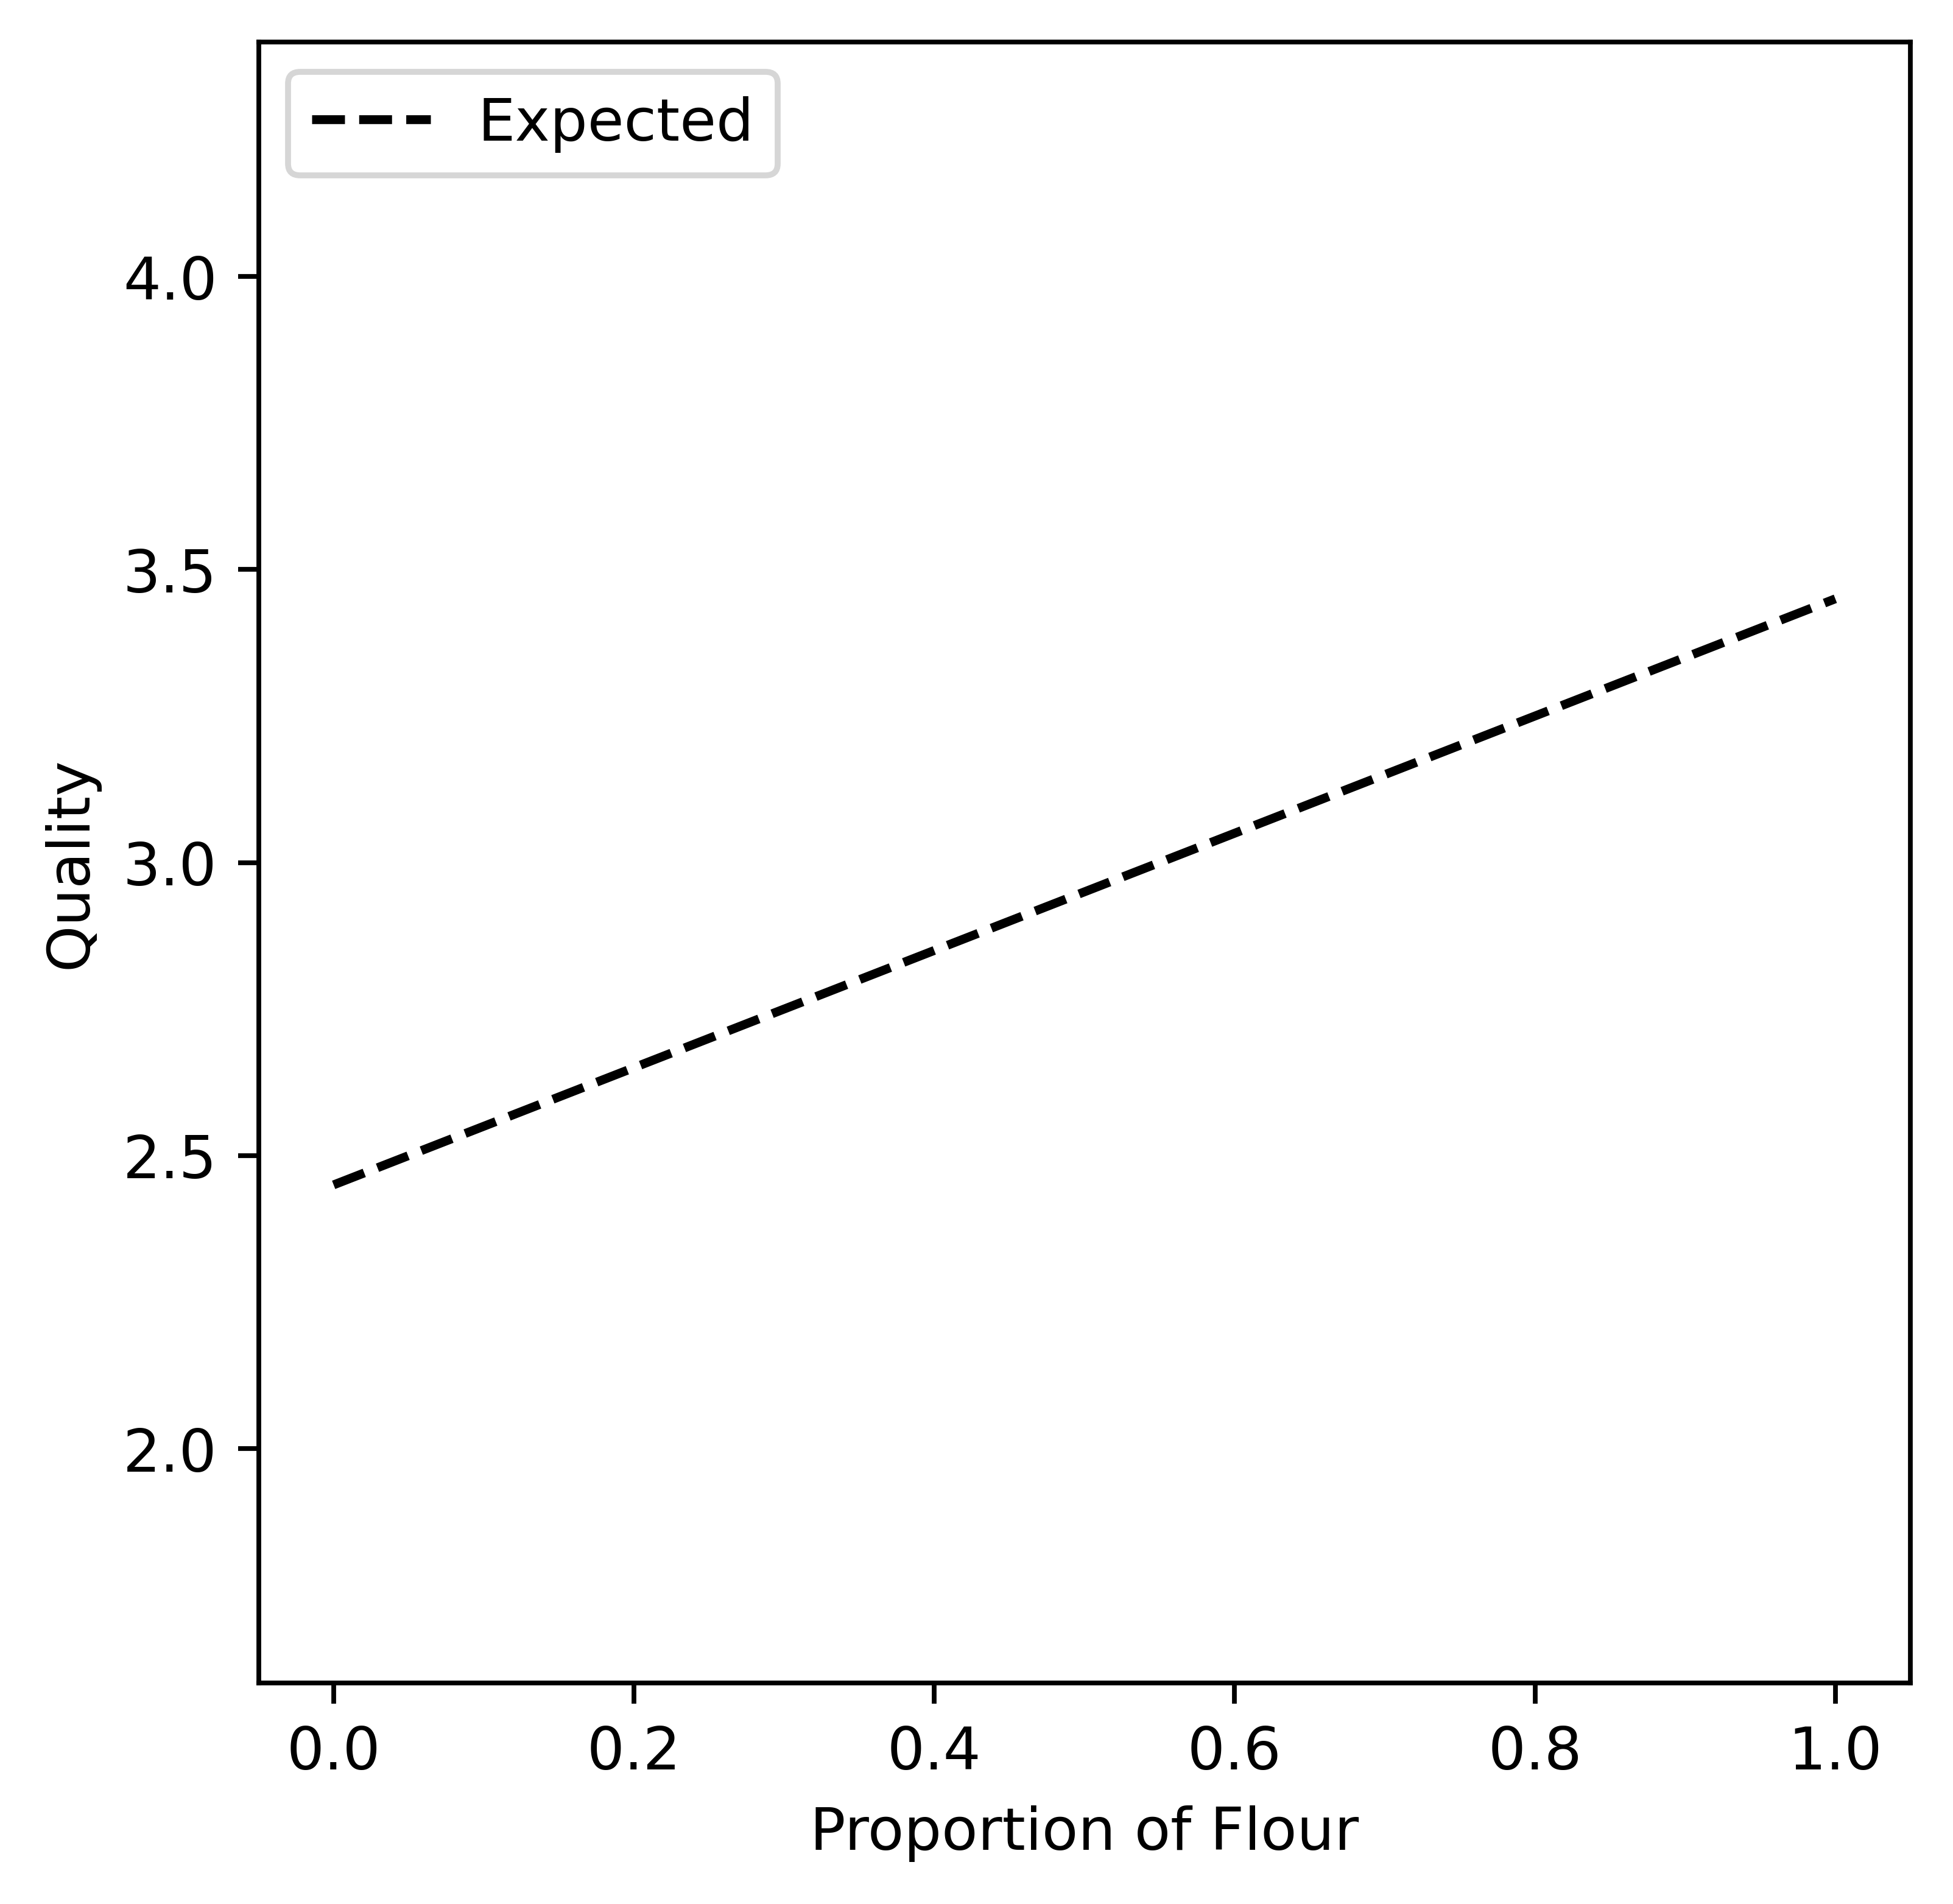
\includegraphics[width=0.5\textwidth]{fig/linear.png}
    \end{center}
\end{frame}

\begin{frame}
    \frametitle{Attempt 2: Quadratic Regression}
    \begin{equation*}
        F(x) = \beta_2 x^2 + \beta_1 x + \beta_0.
    \end{equation*}
    \pause
    \begin{itemize}
        \item  \movie[externalviewer]{Parametric Regression Converges}{../fig/quad-limiting.gif}
            \pause
        \item \movie[externalviewer]{But not always to correctly}{../fig/nonquad-limiting.gif}
    \end{itemize}
\end{frame}

\begin{frame}
    \frametitle{Parametric Forms}
    \begin{equation*}
        \begin{bmatrix}
            F(\mathbf{x}_1) \\
            \vdots \\
            F(\mathbf{x}_N) \\
        \end{bmatrix}
        =
        \begin{bmatrix}
            y_1 \\
            \vdots \\
            y_N
        \end{bmatrix}
        \implies
        \begin{bmatrix}
            \beta_0 \\
            \beta_1 \\
            \beta_2
        \end{bmatrix}
        \implies F
    \end{equation*}
    \pause
    Parametric forms make unjustified assumptions $F$.
\end{frame}

\begin{frame}
    \frametitle{Nonparametric Forms}
    \begin{equation*}
        \begin{bmatrix}
            F(\mathbf{x}_1) \\
            \vdots \\
            F(\mathbf{x}_N) \\
        \end{bmatrix}
        =
        \begin{bmatrix}
            y_1 \\
            \vdots \\
            y_N
        \end{bmatrix}
        \implies F
    \end{equation*}
    \pause
    \begin{enumerate}
        \item The more we sample $F$ ``near'' $\mathbf{x}$, the more confident we are about $F(\mathbf{x})$.
            \pause
        \item If $\mathbf{x}, \mathbf{x}'$ are ``similar'', then $F(\mathbf{x}), F(\mathbf{x}')$ are probably ``similar''.
            \pause
        \item $F$ is smooth.
    \end{enumerate}
\end{frame}

\begin{frame}
    \frametitle{Gaussian Processes}

    Uncountably infinite collection of r.v.
    $\{ F(\mathbf{x}) : \mathbf{x} \in \mathcal{X} \}$.

    \pause
    \begin{definition}[Gaussian Process]
        $F \sim \mathcal{GP}_{ \mathcal{X}}(m, \kappa)$ where
        \begin{align*}
            \mathbb{E}[F(\mathbf{x})] & = m(\mathbf{x}) \\
            \Cov[F(\mathbf{x}), F(\mathbf{x}')] & = \kappa(\mathbf{x}, \mathbf{x}')
        \end{align*}
        with
        \pause
        \begin{equation*}
            \begin{bmatrix}
                F(\mathbf{x}_1) \\
                \vdots \\
                F(\mathbf{x}_K) \\
            \end{bmatrix}
            \sim
            \mathcal{N}_{K}
            \left(
            \begin{bmatrix}
                    m(\mathbf{x}_1) \\
                    \vdots \\
                    m(\mathbf{x}_K) \\
                \end{bmatrix}
            ,
            \begin{bmatrix}
                    \kappa(\mathbf{x}_1, \mathbf{x}_1) & \dots & \kappa(\mathbf{x}_1, \mathbf{x}_K) \\
                    \vdots & \ddots & \vdots \\
                    \kappa(\mathbf{x}_K, \mathbf{x}_1) & \dots & \kappa(\mathbf{x}_K, \mathbf{x}_K) \\
                \end{bmatrix}
            \right).
        \end{equation*}
    \end{definition}
\end{frame}


\end{document}
